\documentclass[12pt]{article}
\usepackage[T1]{fontenc}
\usepackage[T1]{polski}
\usepackage[utf8]{inputenc}
\newcommand{\BibTeX}{{\sc Bib}\TeX} 
\usepackage{graphicx}
\usepackage{amsfonts}
\usepackage{amsmath}
\usepackage{latexsym}
\usepackage{float}

\setlength{\textheight}{21cm}

\title{{\bf Zadanie nr 1 - Generacja sygnału i szumu}\linebreak
Cyfrowe Przetwarzanie Sygnałów}
\author{Dawid Jakubik, 224307 \and Hubert Gawłowski, 224298}
\date{22.04.2021}

\begin{document}
\clearpage\maketitle
\thispagestyle{empty}
\newpage
\setcounter{page}{1}
\section{Cel zadania}

Celem zadania było zapoznanie się z operacjami splotu, filtracji i korelacji sygnałów oraz zaimplementowanie ich rozszerzając tym samym program przygotowany w ramach zadań 1 i 2.

\section{Wstęp teoretyczny}
Podczas pracy nad zadaniem korzystaliśmy z teorii zawartej w intrukcji na platformie Wikamp \cite{instrukcja}. Najważniejsze definicje, jakie trzeba poznać, aby mieć podstawy teoretyczne do zadania dotyczą:
\begin{itemize}
    \item definicji splotu oraz wzoru na niego
    \item definicji korelacji oraz wzoru na korelację bezpośrenią oraz z użyciem splotu
    \item definicji filtracji, filtru dolnoprzepustowego oraz okna prostokątnego, a także wzorów na okna: Hamminga, Hanninga i Blackmana oraz filtrów: śtodkowoprzepustowego i górnoprzepustowego
    \item definicji odpowiedzi impulsowej filtru
\end{itemize}
W ramach zadania, zgodnie z poleceniem poza oknem prostokątnym zaimplementowaliśmy okno Hanninga, a oprócz filtru dolnoprzepustowego został zaimplementowany filtr środkowoprzepustowy.

\section{Eksperymenty i wyniki}

%%%%%%%%%%%%%%%%%%%%%%%%%%%%%%%%%%%%%%%%%%%%%%%%%%%%%%%%%%%%%%%%%%%%%%%%%%%%%%%%%%%%%%%%%%%%%%%%%%%%%%%%%%%%%%%%%
% PODROZDZIA£ PT. EKSPERYMENT NR 1 
%%%%%%%%%%%%%%%%%%%%%%%%%%%%%%%%%%%%%%%%%%%%%%%%%%%%%%%%%%%%%%%%%%%%%%%%%%%%%%%%%%%%%%%%%%%%%%%%%%%%%%%%%%%%%%%%%

\subsection{Splot sygnałów dyskretnych}

Pierwsza pula eksperymentów miała na celu pokazanie splotu sygnałów dyskretnych

\subsubsection{Eksperyment nr 1: Splot sygnałów sinusoidalnych}

W pierwszym eksperymencie dokonaliśmy operacji splotu na dwóch sygnałach sinusoidalnych o następujących parametrach:
\begin{itemize}
    \item Dla sygnału pierwszego: 
    \begin{itemize}
        \item Amplituda: 5
        \item Start w sekundzie: 0
        \item Czas trwania w sekundach: 3
        \item Okres podstawowy: 2
        \item Częstotliwość próbkowania: 70
    \end{itemize}
    \item Dla sygnału drugiego:
    \begin{itemize}
        \item Amplituda: 5
        \item Start w sekundzie: 1
        \item Czas trwania w sekundach: 3
        \item Okres podstawowy: 2
        \item Częstotliwość próbkowania: 70
    \end{itemize}
\end{itemize}
Sygnały wejściowe prezentują się następująco:
\begin{figure}[H]
    \centering
    %\includegraphics{cps_kwantyzacja_z_obcieciem_miary.jpg}
	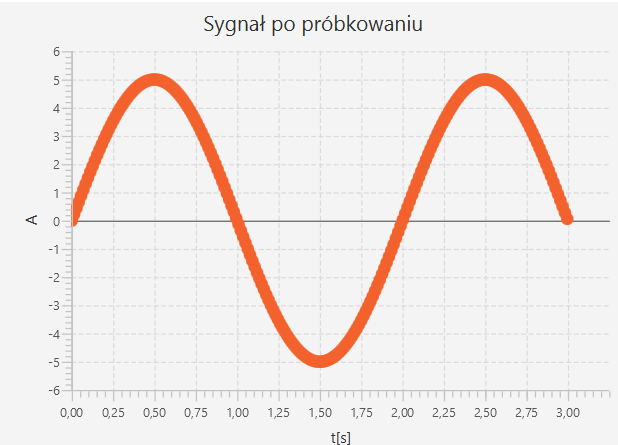
\includegraphics[width=\linewidth]{sygnal_po_probkowaniu_1.1.png}
    \caption{Sygnał nr 1, który zostanie poddany operacji splotu}
    \label{Sygnał_1.1}
\end{figure}

\begin{figure}[H]
    \centering
    %\includegraphics{cps_kwantyzacja_z_obcieciem_miary.jpg}
	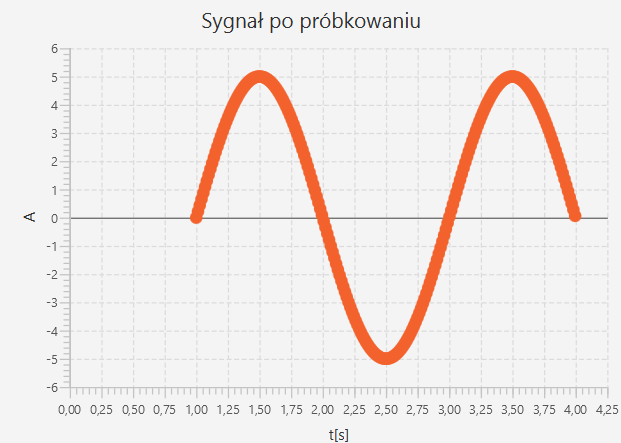
\includegraphics[width=\linewidth]{sygnal_po_probkowaniu_1.2.png}
    \caption{Sygnał nr 2, który zostanie poddany operacji splotu}
    \label{Sygnał_1.2}
\end{figure}

Wynik operacji splotu dwóch powyższych sygnałów przedstawia się następująco
\begin{figure}[H]
    \centering
    %\includegraphics{cps_kwantyzacja_z_obcieciem_miary.jpg}
	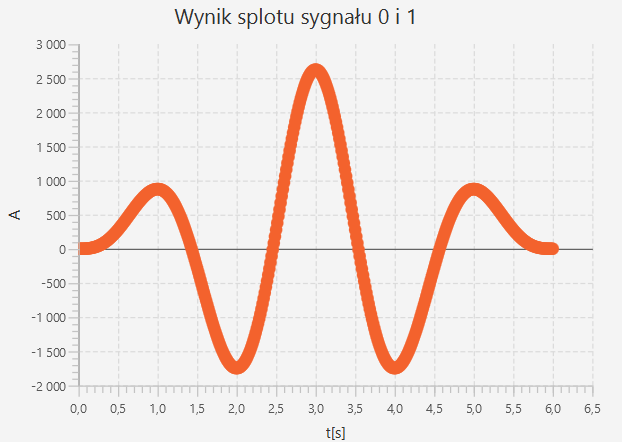
\includegraphics[width=\linewidth]{splot_1.1.png}
    \caption{Wynik operacji splotu sygnałów z rysunków \ref{Sygnał_1.1} i \ref{Sygnał_1.2}}
    \label{Wynik_1.1}
\end{figure}

%%%%%%%%%%%%%%%%%%%%%%%%%%%%%%%%%%%%%%%%%%%%%%%%%%%%%%%%%%%%%%%%%%%%%%%%%%%%%%%%%%%%%%%%%%%%%%%%%%%%%%%%%%%%%%%%%

%%%%%%%%%%%%%%%%%%%%%%%%%%%%%%%%%%%%%%%%%%%%%%%%%%%%%%%%%%%%%%%%%%%%%%%%%%%%%%%%%%%%%%%%%%%%%%%%%%%%%%%%%%%%%%%%%

\subsubsection{Eksperyment nr 2: Splot sygnałów sinusoidalnego wyprostowanego jednopółkowo oraz sygnału trójkątnego}

W kolejnym eksperymencie wykonaliśmy splot na sygnałach sinusoidalnym wyprostowanym jednopółkowym oraz trójkątnym. Sygnały przyjęły następujące parametry:

\begin{itemize}
    \item Dla sygnału pierwszego (sinusoidalnego jednopółkowego): 
    \begin{itemize}
        \item Amplituda: 3
        \item Start w sekundzie: 1
        \item Czas trwania w sekundach: 4
        \item Okres podstawowy: 1
        \item Częstotliwość próbkowania: 50
    \end{itemize}
    \item Dla sygnału drugiego (trójkątnego):
    \begin{itemize}
        \item Amplituda: 2
        \item Start w sekundzie: 1
        \item Czas trwania w sekundach: 4
        \item Okres podstawowy: 3
        \item Współczynnik wypełnienia: 0.4
        \item Częstotliwość próbkowania: 50
    \end{itemize}
\end{itemize}
Sygnały wejściowe prezentują się następująco:
\begin{figure}[H]
    \centering
    %\includegraphics{cps_kwantyzacja_z_obcieciem_miary.jpg}
	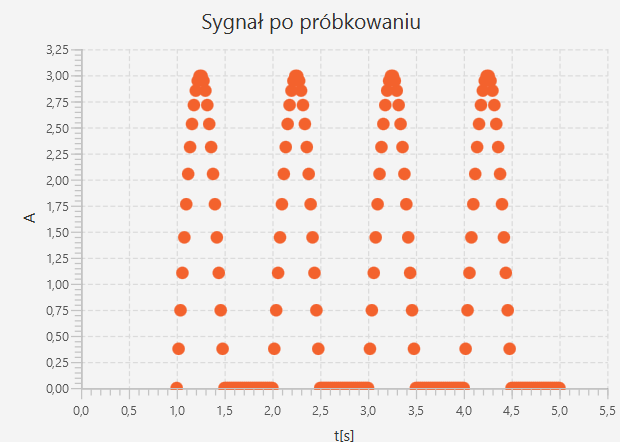
\includegraphics[width=\linewidth]{sygnal_po_probkowaniu_2.1.png}
    \caption{Sygnał nr 1, który zostanie poddany operacji splotu}
    \label{Sygnał_2.1}
\end{figure}

\begin{figure}[H]
    \centering
    %\includegraphics{cps_kwantyzacja_z_obcieciem_miary.jpg}
	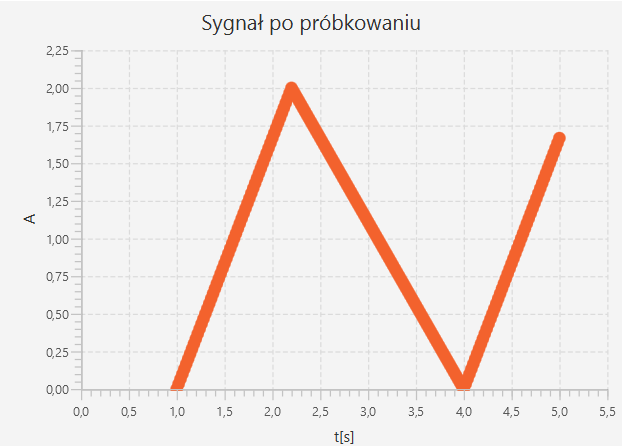
\includegraphics[width=\linewidth]{sygnal_po_probkowaniu_2.2.png}
    \caption{Sygnał nr 2, który zostanie poddany operacji splotu}
    \label{Sygnał_2.2}
\end{figure}

Wynik operacji splotu dwóch powyższych sygnałów przedstawia się następująco
\begin{figure}[H]
    \centering
    %\includegraphics{cps_kwantyzacja_z_obcieciem_miary.jpg}
	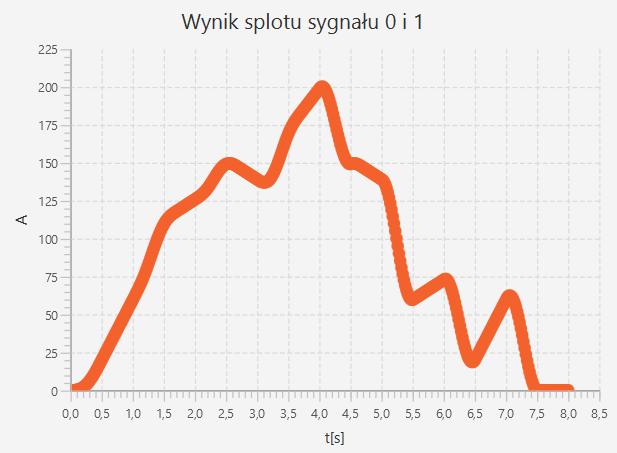
\includegraphics[width=\linewidth]{splot_2.1.png}
    \caption{Wynik operacji splotu sygnałów z rysunków \ref{Sygnał_2.1} i \ref{Sygnał_2.2}}
    \label{Wynik_2.1}
\end{figure}

%%%%%%%%%%%%%%%%%%%%%%%%%%%%%%%%%%%%%%%%%%%%%%%%%%%%%%%%%%%%%%%%%%%%%%%%%%%%%%%%%%%%%%%%%%%%%%%%%%%%%%%%%%%%%%%%%

%%%%%%%%%%%%%%%%%%%%%%%%%%%%%%%%%%%%%%%%%%%%%%%%%%%%%%%%%%%%%%%%%%%%%%%%%%%%%%%%%%%%%%%%%%%%%%%%%%%%%%%%%%%%%%%%%

\subsubsection{Eksperyment nr 3:  Splot sygnałów trójkątnego oraz sinusoidalnego wyprostowanego jednopółkowo}
W kolejnym eksperymencie przeprowadziliśmy splot na takich samych sygnałach jak w eksperymencie powyżej, jednak zmieniliśmy kolejność sygnałów - w tym przypadku sygnałem nr 1 będzie sygnał trójkątny, a sygnałem nr 2 - sygnał sinusoidalny jednopółkowy. Celem tego eksperymentu jest zbadanie, czy wzór (2) podany w instrukcji do zadania \cite{instrukcja} jest przemienny tzn. czy (h*x)(n) da nam ten sam wynik, co (x*h)(n). Tak więc - podsumowując do eksperymentów wykorzystamy następujące z następującymi parametrami:
\begin{itemize}
    \item Dla sygnału pierwszego (trójkątnego):
    \begin{itemize}
        \item Amplituda: 2
        \item Start w sekundzie: 1
        \item Czas trwania w sekundach: 4
        \item Okres podstawowy: 3
        \item Współczynnik wypełnienia: 0.4
        \item Częstotliwość próbkowania: 50
    \end{itemize}
    \item Dla sygnału drugiego (sinusoidalnego jednopółkowego): 
    \begin{itemize}
        \item Amplituda: 3
        \item Start w sekundzie: 1
        \item Czas trwania w sekundach: 4
        \item Okres podstawowy: 1
        \item Częstotliwość próbkowania: 50
    \end{itemize}
\end{itemize}
Sygnały wejściowe prezentują się następująco:
\begin{figure}[H]
    \centering
    %\includegraphics{cps_kwantyzacja_z_obcieciem_miary.jpg}
	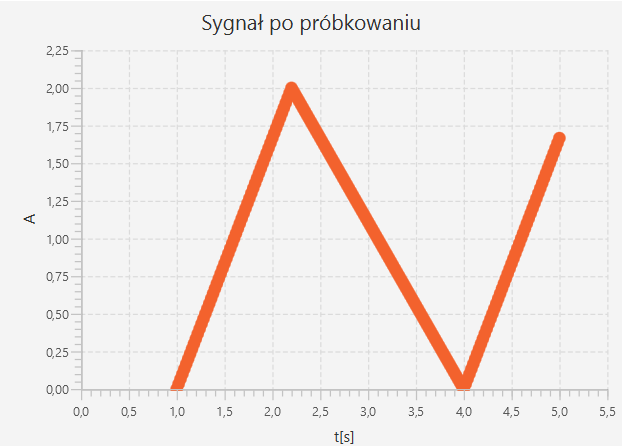
\includegraphics[width=\linewidth]{sygnal_po_probkowaniu_2.2.png}
    \caption{Sygnał nr 1, który zostanie poddany operacji splotu}
    \label{Sygnał_3.1}
\end{figure}

\begin{figure}[H]
    \centering
    %\includegraphics{cps_kwantyzacja_z_obcieciem_miary.jpg}
	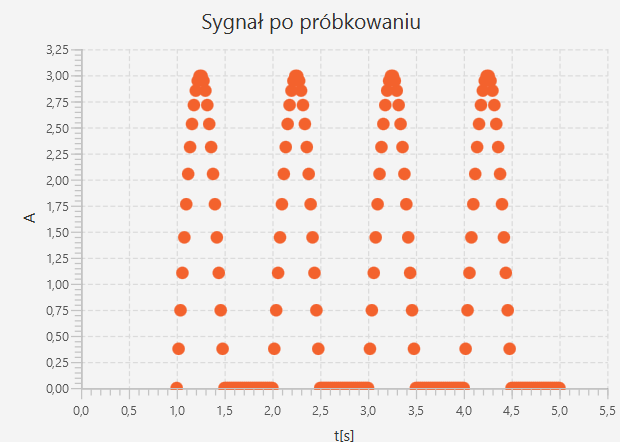
\includegraphics[width=\linewidth]{sygnal_po_probkowaniu_2.1.png}
    \caption{Sygnał nr 2, który zostanie poddany operacji splotu}
    \label{Sygnał_3.2}
\end{figure}

Wynik operacji splotu dwóch powyższych sygnałów przedstawia się następująco
\begin{figure}[H]
    \centering
    %\includegraphics{cps_kwantyzacja_z_obcieciem_miary.jpg}
	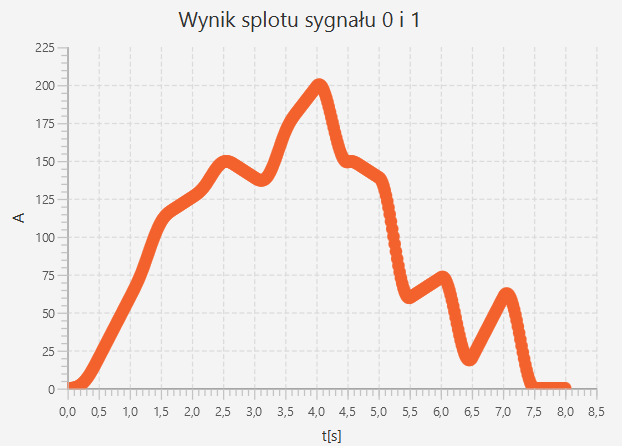
\includegraphics[width=\linewidth]{splot_3.1.png}
    \caption{Wynik operacji splotu sygnałów z rysunków \ref{Sygnał_3.1} i \ref{Sygnał_3.2}}
    \label{Wynik_3.1}
\end{figure}

%%%%%%%%%%%%%%%%%%%%%%%%%%%%%%%%%%%%%%%%%%%%%%%%%%%%%%%%%%%%%%%%%%%%%%%%%%%%%%%%%%%%%%%%%%%%%%%%%%%%%%%%%%%%%%%%%

%%%%%%%%%%%%%%%%%%%%%%%%%%%%%%%%%%%%%%%%%%%%%%%%%%%%%%%%%%%%%%%%%%%%%%%%%%%%%%%%%%%%%%%%%%%%%%%%%%%%%%%%%%%%%%%%%
\newpage
\subsubsection{Eksperyment nr 4: Splot sygnałów prostokątnego i sinusoidalnego wyprostowanego dwupółkowo}
W tym eksperymencie dokonaliśmy splotu na sygnałach prostokątym oraz sinusoidalnym dwupółkowym o następujących parametrach:
\begin{itemize}
    \item Dla sygnału pierwszego (prostokątnego):
    \begin{itemize}
        \item Amplituda: 4
        \item Start w sekundzie: 0
        \item Czas trwania w sekundach: 4
        \item Okres podstawowy: 2
        \item Współczynnik wypełnienia: 0.6
        \item Częstotliwość próbkowania: 10
    \end{itemize}
    \item Dla sygnału drugiego (sinusoidalnego dwupółkowego): 
    \begin{itemize}
        \item Amplituda: 1 
        \item Start w sekundzie: 0 
        \item Czas trwania w sekundach: 4
        \item Okres podstawowy: 4
        \item Częstotliwość próbkowania: 20
    \end{itemize}
\end{itemize}
Sygnały wejściowe prezentują się następująco:
\begin{figure}[H]
    \centering
    %\includegraphics{cps_kwantyzacja_z_obcieciem_miary.jpg}
	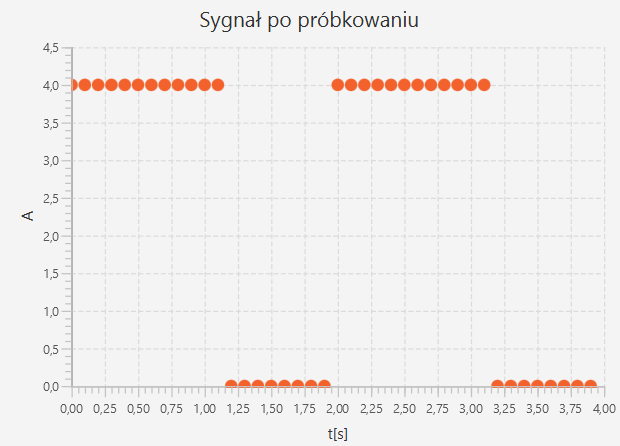
\includegraphics[width=\linewidth]{sygnal_po_probkowaniu_4.1.png}
    \caption{Sygnał nr 1, który zostanie poddany operacji splotu}
    \label{Sygnał_4.1}
\end{figure}

\begin{figure}[H]
    \centering
    %\includegraphics{cps_kwantyzacja_z_obcieciem_miary.jpg}
	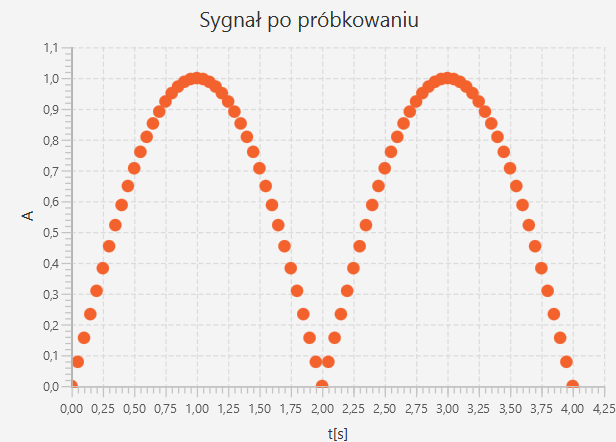
\includegraphics[width=\linewidth]{sygnal_po_probkowaniu_4.2.png}
    \caption{Sygnał nr 2, który zostanie poddany operacji splotu}
    \label{Sygnał_4.2}
\end{figure}

Wynik operacji splotu dwóch powyższych sygnałów przedstawia się następująco
\begin{figure}[H]
    \centering
    %\includegraphics{cps_kwantyzacja_z_obcieciem_miary.jpg}
	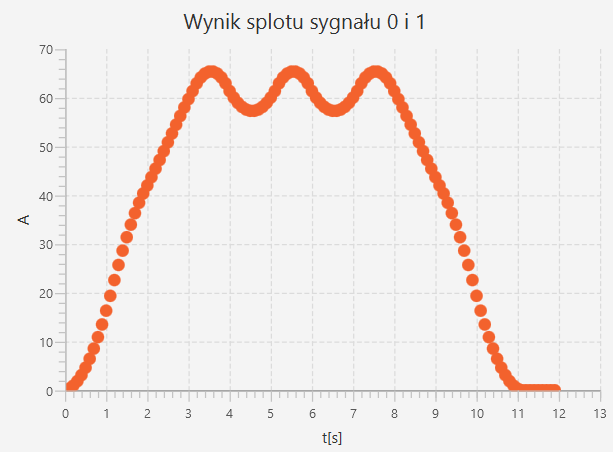
\includegraphics[width=\linewidth]{splot_4.1.png}
    \caption{Wynik operacji splotu sygnałów z rysunków \ref{Sygnał_4.1} i \ref{Sygnał_4.2}}
    \label{Wynik_4.1}
\end{figure}


\section{Wnioski}
Program umożliwia generowanie wykresów będącymi wynikami operacji splotu, korelacji oraz filtracji.
\subsection{Splot sygnałów dyskretnych}
Pierwsza pula eksperymentów polegała na splocie sygnałów dyskretnych. W eksperymencie nr 1 dokonaliśmy operacji splotu na takich samych sygnałach sinusoidalnych, przesuniętych w czasie o 1 s. Wynik operacji splotu jest zgodny z założeniami. Sygnał wynikowy ma okres równy sumie okresów obu sygnałów. Pozwala nam to wysnuć wniosek, że przesunięcie w czasie nie ma wpływu na operacje splotu. W eksperymencie 2, w którym dokonaliśmy operacji splotu dla sygnałów sinusoidalnego wyprostowanego jednopółkowo oraz trójkątnego wyniki również wydają się logiczne i sensowne. Długość trwania sygnału splotu odpowiada sumie długości trwania sygnałów wejściowych, a maksymalną wartość splot przyjmuje dokładnie w połowie czasu trwania. Następny eksperyment (nr 3) dowodzi, że operacja splotu jest przemienna tzn. bez względu, który sygnał przyjmiemy jako h, a który jako x we wzorze na splot \cite{instrukcja} - wynik będzie taki sam. Eksperyment 4 przeprowadziliśmy dla typów sygnałów, dla których wcześniej nie przeprowadzaliśmy eksperymentów oraz z zdecydowanie mniejszą (i różną od siebie) częstotliwością próbkowania. Wynik pokazuje, że przy operacji splotu częstotliwość próbkowania obu sygnałów dyskretnych nie musi być taka sama.

 

%%%%%%%%%%%%%%%%%%%%%%%%%%%%%%%%%%%%%%%%%%%%%%%%%%%%%%%%%%%%%%%%%%%%%%%%%%%%%%%%%%%%%%%%%%%%%%%%%%%%%%%%%%%%%%%%%
% BIBLIOGRAFIA
%%%%%%%%%%%%%%%%%%%%%%%%%%%%%%%%%%%%%%%%%%%%%%%%%%%%%%%%%%%%%%%%%%%%%%%%%%%%%%%%%%%%%%%%%%%%%%%%%%%%%%%%%%%%%%%%%
\begin{thebibliography}{}
\bibitem{instrukcja} Instrukcja do zadania 3 na stronie przedmiotu. [przeglądany 26.05.2021], Dostępny w: https://ftims.edu.p.lodz.pl/pluginfile.php/14039/mod\_resource/content/1/zad3.pdf


\end{thebibliography}



\end{document}
